\subsection{Время и USB-энергия на общих 500 потоках}
\label{sec:hw500}
Методические ориентиры измерения энергии встроенного ML задают MLPerf Tiny~\cite{Banbury2021MLPerfTiny} и ULPMark-CoreMark~\cite{EEMBCULPMarkCM}. Здесь используются длительные повторяемые партии и энергия того же интервала, но иной состав нагрузки и собственный измерительный тракт. Соблюдение стандартного бенчмарка или сертификация ULPMark не заявляются. USB-тестер FNIRSI FNB58 (серийный номер 104332) включён последовательно в питание платы; фотографии на рис.~\ref{fig:energy-setup} иллюстрируют установку.

\begin{figure}[!htbp]
\centering
\begin{minipage}[t]{0.46\textwidth}
\centering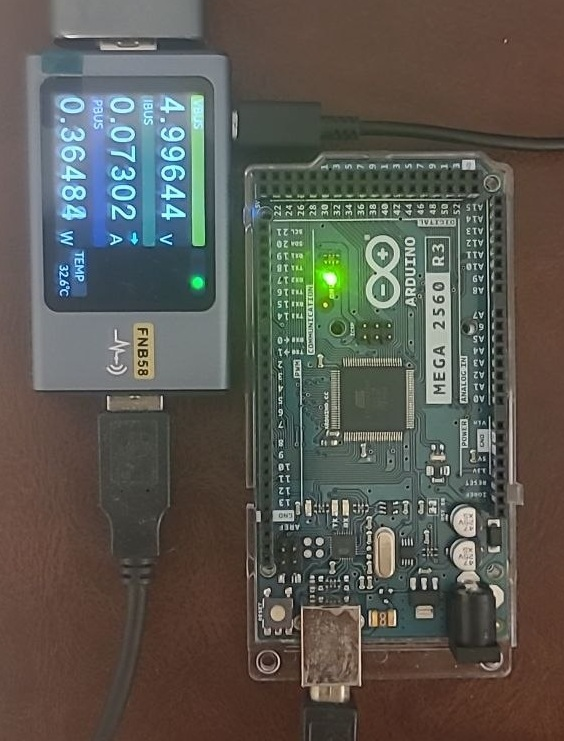
\includegraphics[height=5cm]{figures/Mega_measurement.jpg}\\[2pt]
\small (a) Arduino Mega 2560
\end{minipage}\hfill
\begin{minipage}[t]{0.46\textwidth}
\centering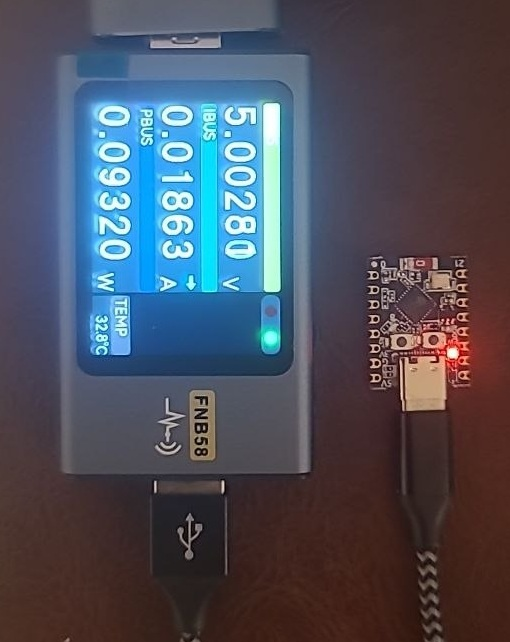
\includegraphics[height=5cm]{figures/C3_measurement.jpg}\\[2pt]
\small (b) ESP32-C3
\end{minipage}
\caption{Подключение плат к USB-тестеру FNB58. Фотографии иллюстрируют измерительную установку; показания на экранах являются отдельными снимками и не представляют средние активных вычислительных интервалов. Исполненная прошивка, модель и идентификатор платы устанавливаются по журналам и двоичным файлам, а не по фотографиям.}
\label{fig:energy-setup}
\end{figure}


\paragraph{Общая нагрузка для времени и энергии.}
Для измерения времени и энергии на прежних платах Mega 2560 и ESP32-C3 использована одна когорта из 500 потоков: 250 нормальных и 250 атакующих. Измерялись прежние замороженные модели; новые модели, обученные на непересекающемся по парам разбиении, в эту аппаратную серию не экспортировались. На каждой плате выполнены отдельный коэффициентный пилот и пять блоков по пять моделей с заранее заданной циклической перестановкой порядка. Получено по пять технических повторов каждой конфигурации; пилот исключён из средних. Перед каждым опытом выполнялись новая загрузка и перезапуск, 500 прогревочных предсказаний, подбор числа проходов для активного окна около 120\,с и не менее 30\,с стабилизации. Подготовленная строка считывалась из Flash в небольшой буфер RAM, затем выполнялись предсказание и накопление контрольной суммы. Из активного окна исключены извлечение признаков, захват пакетов, последовательный вывод, светодиодные маркеры, прогрев и подбор числа проходов. На C3 частота CPU равна 160~МГц, прерывания разрешены, явного \texttt{yield} внутри активной партии нет. Длительность блока, делённая на число предсказаний, характеризует среднее время обработки в блоке, а не распределение задержек отдельных запросов.

\paragraph{Совмещение временных шкал и расчёт энергии.}
На каждой плате один непрерывный файл FNB58 охватывал пилот и 25 основных опытов. Группы светодиодных импульсов до и после каждого опыта сопоставлялись с журналом времени компьютера; аффинная подгонка двенадцати фронтов с метками MCU связывала активное окно с записью мощности. Интеграл VBUS$\times$IBUS вычислялся методом трапеций и делился на фактическое число предсказаний. Поэтому время и энергия в табл.~\ref{tab:hw500-energy} относятся к одному блоку, а энергия включает всю плату и соединение после USB-измерителя. Мощность соседних интервалов ожидания сохранена для диагностики, но не вычитается. Для четырёх конфигураций Mega знаковая разность после такого вычитания отрицательна; её нельзя интерпретировать как отрицательную энергию предсказания. Необъяснённое расхождение канала NRG, составляющего около четверти интеграла VBUS$\times$IBUS, сохранено в материалах. Этот канал не используется и не пересчитывается эмпирическим множителем.

Для соответствующих границ активной партии $a$ и $b$ на оси времени CFN имеем
\begin{equation}
\widehat E_{\rm iter}=\frac{1}{N}\int_a^b V(t)I(t)\,dt,
\qquad \overline t_{\rm iter}=\frac{T_{\rm MCU}}{N}.
\label{eq:hw500-energy}
\end{equation}
Здесь $N$ --- число завершённых предсказаний; интеграл вычисляется с линейной интерполяцией на границах окна. Это энергия всей измеряемой итерации, а не разрешённая прибором микросекундная форма импульса одного ядра.

\begin{table}[!htbp]
\centering\small\setlength{\tabcolsep}{7pt}
\caption{Общая нагрузка из 500 потоков: среднее время и USB-энергия всей платы на одну итерацию, рассчитанные по одному и тому же полному активному блоку. Для каждой модели и платы выполнено пять технических повторов; энергия представлена как среднее $\pm$ выборочное SD. Отдельный коэффициентный пилот исключён. Число знаков отражает сохранённую повторяемость, а не абсолютную точность прибора.}
\label{tab:hw500-energy}
\begin{tabular}{lrrrr}
\toprule
Модель & \multicolumn{2}{c}{Mega 2560} & \multicolumn{2}{c}{ESP32-C3} \\
 & Время (мкс) & Энергия (мкДж) & Время (мкс) & Энергия (мкДж) \\
\midrule
KAN, коэффициенты & 1412.4 & $498.4\pm0.8$ & 5.892 & $0.9874\pm0.0004$ \\
KAN, LUT & 258.83 & $92.16\pm0.13$ & 4.961 & $0.8590\pm0.0007$ \\
MLP16 & 1344.4 & $477.3\pm0.7$ & 20.592 & $3.5263\pm0.0040$ \\
Многослойная KAN & 12321.8 & $4367\pm4$ & 55.752 & $9.6408\pm0.0102$ \\
DT5 & 33.035 & $11.884\pm0.010$ & 1.536 & $0.2643\pm0.0002$ \\
\bottomrule
\end{tabular}
\end{table}


\paragraph{Результаты и интерпретация.}
LUT сократил среднее время блока относительно коэффициентного KAN в 5,457 раза на Mega и в 1,188 раза на C3; отношения USB-энергии составили соответственно 5,407 и 1,149. DT5 остался самым быстрым и наименее энергозатратным из исследованных вариантов. Для каждой конфигурации Mega все пять сохранённых длительностей совпали. Это нулевой наблюдаемый разброс значений длительности блока, а не нулевая погрешность времени. Новая серия устраняет различие нагрузки между прежними энергетическими пилотами на двадцати потоках и временными опытами на 500 потоках. Исторические протоколы сохранены отдельно и не объединяются с новой серией. Результат C3 не устанавливает причину прежнего замедления LUT на 7,58\% при другом протоколе.

\paragraph{Границы измерений.}
Независимая калибровка измерителя и часов не проводилась. Сетка хранения 0,1\,с не означает полосу измерения 10\,Гц: наблюдаемый отклик на маркеры составляет около 1\,с. Максимальная невязка подгонки фронтов меньше 0,102\,с на Mega и 0,143\,с на C3. Общий сдвиг обоих концов окна в пределах $\pm2$\,с изменял оценки не более чем на 0,034\% и 0,605\% соответственно. Эти величины служат диагностикой совмещения, а не полным бюджетом неопределённости. Среднее и выборочное SD характеризуют техническую повторяемость на одном экземпляре каждой платы и не оценивают абсолютную точность, различия между экземплярами, изолированную энергию процессора или полные затраты IDS.
